\section{H16: Idle traps deepen with time}
\label{sec:H16}

\textbf{The question:} Agents sometimes get stuck in long silences, chains of timer pauses or repeated failures. Is the escape from such a trap memoryless, as Kramers escape predicts, or does the trap deepen with time? What gets a stuck agent out?

\textbf{The intuition:} In the Kramers picture, noise kicks a particle over the barrier of its well. It escapes at a constant rate, whatever time it has already spent there: the escape is memoryless. In the aging picture (a Bouchaud trap model), trap depths have a broad spread. The longer an agent stays stuck, the more likely it sits in a deep trap. The hazard, the chance of escape per unit time for an agent still stuck, then falls with time. A kick is a message to the agent. In Kramers, each kick lowers the barrier, so escape rises exponentially with the number of kicks. In the rival picture, the agent reads the kick at its next call, so the first kick does the work and more kicks add little.

\begin{figure}[h]
\includegraphics[width=\textwidth]{H16-trap-aging/fig.pdf}
\caption{Idle traps age by themselves, and one directed kick helps. (a) Simulation: with one trap depth the escape chance does not depend on trap age, but with a broad spread of depths it falls. (b) In \#51, fewer pause points start a run of activity as the trap ages, with a directed message (orange) or without one (dark). (c) Aging slopes in four goal periods stay negative when an input-starvation clock enters the model. Animation: \texttt{writeup/visuals/H16-trap-aging/anim.mp4}.}
\label{fig:int-H16}
\end{figure}
\begin{figure}[h]
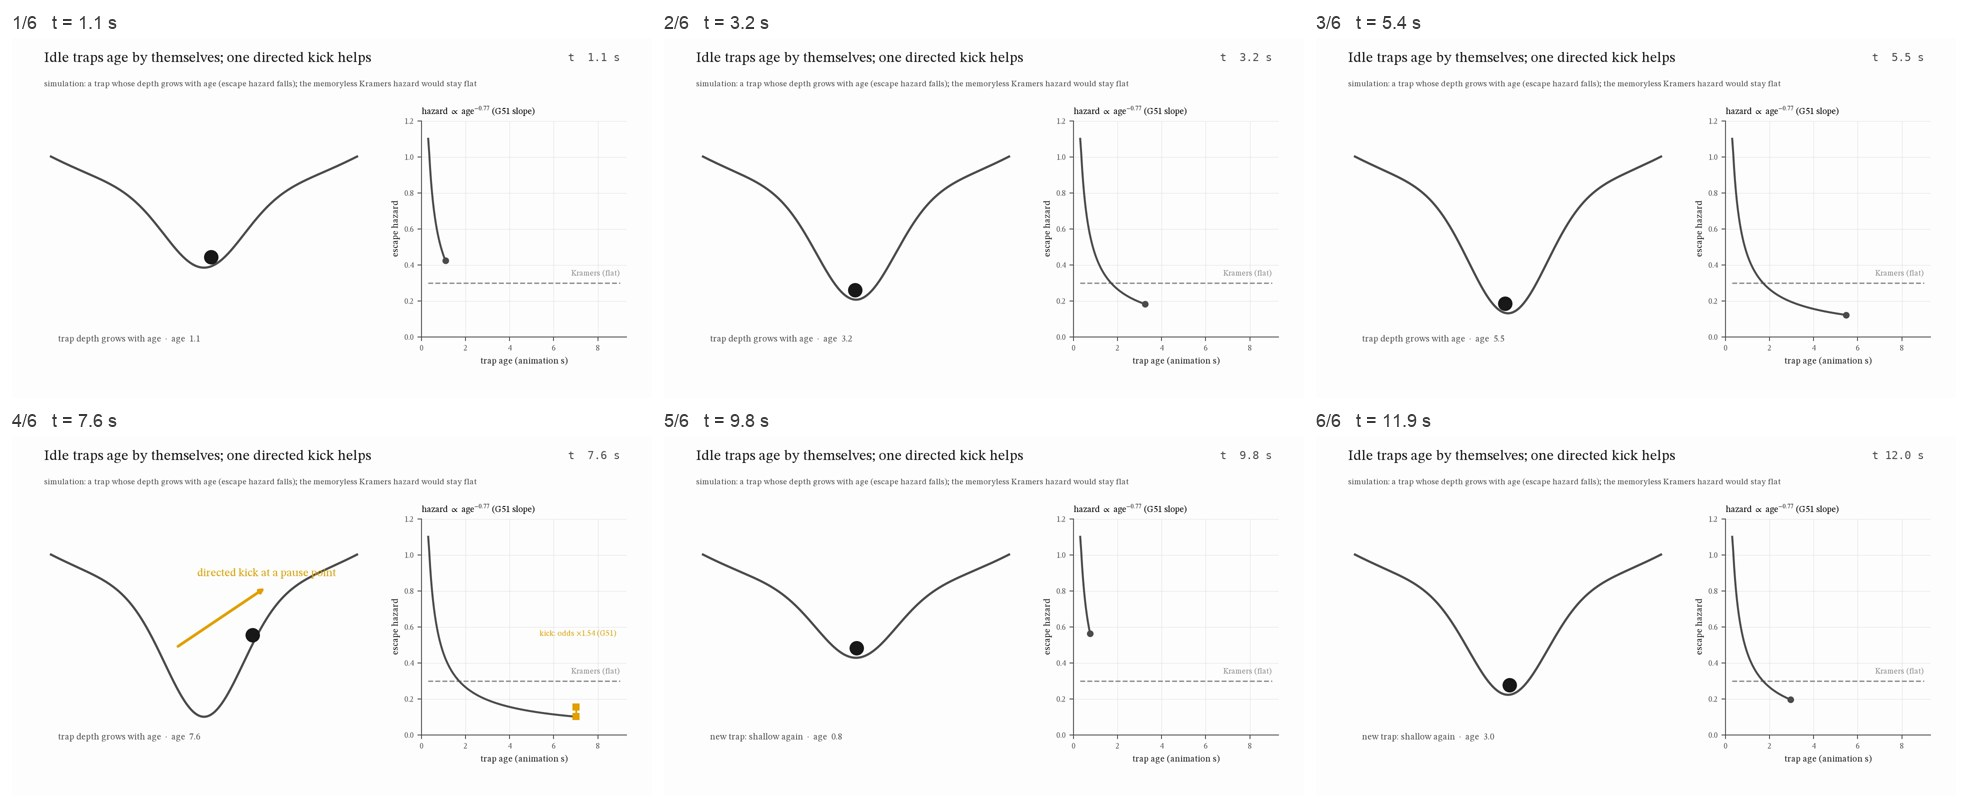
\includegraphics[width=0.9\textwidth]{storyboards/H16.jpg}
\caption{Animation storyboard: six frames of the animation, evenly spaced in time (frame number and time above each). The full animation is \texttt{writeup/visuals/H16-trap-aging/anim.mp4}.}
\end{figure}


\textbf{What we measured:} Inactive spells are gaps of 180\,s or more; single isolated actions do not end them. Pause chains are runs of timer pauses, with one decision at each timer wake. The hazard slope $\beta$ on $\ln(\text{time elapsed})$ uses spells of 10\,min or more, with agent fixed effects: $\beta=0$ is memoryless, $\beta<0$ is aging, and $|\beta|\le0.3$ counts as memoryless. At each timer wake, a logit relates the chance to act to the chain length. A kick is a directed message in the prior 2\,min; the null takes the same agent's kicks from another day. Impostors: agent fixed effects and the day-swap null partly remove the scheduler field. Past-only kicks remove the external drive, and the aging persists with the nudger off (NE43). The shared model prior is not relevant: fixed effects absorb each agent's frailty, and the card makes no family claim. Common input is open, because kicks count by posting time, not by the read-out call. The synthetic check used overdamped Langevin agents seen through event times. Memoryless truth gave $+0.05\pm0.07$; deepening traps gave $-0.58$ and $-1.08$ (truth $-0.54$, $-1.18$). Without fixed effects, frailty alone faked aging of $-0.25$.

\textbf{What we found:} Within an agent, escape from inactive spells and pause chains ages instead of being memoryless\cred{0.70}; EU 2.1 (value if true 3.0). The inactive-spell slope is $-0.77$ $[-0.81,-0.73]$ in \#51 (4,321 escapes) and $-1.71$ in \#38. It is below $-0.3$ in 6/8 regime-III goal periods, but its interval lies below $-0.3$ in only 3/8. The chance to act at a timer wake falls with chain length in 6/7 periods (\#51 $-0.38$). With the nudger off (NE43), the aging does not change ($-0.59\to-0.53$). One directed message during a pause raises the odds of acting at the next timer wake $\times1.5$--$2.9$ in 5/7 periods (\#51 $\times1.54$). The dose response is additive or saturating in 14/16 powered cells, not exponential. On real failures, error-loop aging survives only in \#51 ($-0.57$), and messages do not break failure loops (9/9 periods). The mean-field coupling $\beta J_0$ is 0.09--0.41, so the swarm has no collective bistability. The scope is 11 goal periods (8 in regime III), silences and pause chains only. The credence comes from an adjudication: the coordinator gave a wider claim 0.44 and marked it fragile; the blind rater's 0.70 stood, not fragile.

\textbf{What it means:} For an operator, kick a stuck agent early, because its escape hazard falls roughly as $t^{-0.8}$. Send one directed message during a pause. Under the 5-min pause default, it lifts escape from deep pause chains from 0.17 to 0.25; before that default (NE44), from 0.21 to 0.56. A second message adds little. For an agent in a real failure loop, use tooling or a reset, not messages.

\textbf{Caveats:} Spells of different kinds within one agent can mimic aging, and fixed effects remove only differences between agents. The pre-registered count rule (5/8 periods) is not met, and short periods give unstable bootstrap intervals. The predicted drop in the chance to act with the nudger off failed ($+0.006$ $[-0.09, 0.10]$), and so did the NE44 interaction as stated. We defined the robust pause-chain rule after we saw the data. No confirmation test on reserved goal periods has run. Figure panels (b) and (c) use H72's estimator, whose \#51 aging slope is $-0.48$, not $-0.77$.
